% LM_C4-134-152 (scans 134-152), second pass: checked line by line against the scans; changes in LM_C4-134-152_changes.md
\scanpage{134}

\margin{\figure{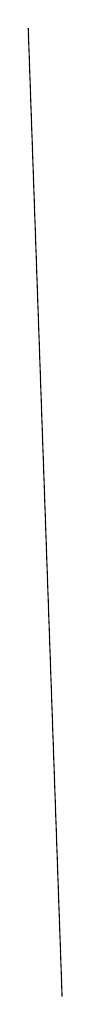
\begin{tikzpicture}\draw (0,0) -- (0.43,-12.3);\end{tikzpicture}}}

de $\mathcal M$ satisfaisant aux conditions suivantes

\par a) $M\longrightarrow\widetilde{\widetilde{\mathcal M}}$ (\unsure{composé} $M\longrightarrow\widetilde{\mathcal M}\longrightarrow\widetilde{\widetilde{\mathcal M}}$) est injectif,

\par \deleted{b) $\unsure{\Gamma'}\ \widetilde{\widetilde{\mathcal M}}/\unsure{M|\Gamma}$}

\par d'où extension

\par $(293)$\quad
\diagram{\begin{tikzcd}[ampersand replacement=\&,column sep=small]
1\arrow[r,dash]\&M\arrow[r,dash]\&\widetilde{\widetilde{\mathcal M}}\arrow[r,dash]\&\deleted{\unsure{\widetilde{\widetilde{\mathcal M}}/M}}\,\underset{\inserted{\overset{\mathrm{dfn}}{=}\widetilde{\widetilde{\mathcal M}}/M}}{\Gamma'}\arrow[r,dash]\&1
\end{tikzcd}}

\par b) \deleted{$\unsure{\widetilde{\widetilde{\mathcal M}}/M}$} $\Gamma'\overset{\mathrm{dfn}}{=}\widetilde{\widetilde{\mathcal M}}/M$ opère \uline{\unsure{fidèlement}} sur $M$,

\par i.e. on a
\[
\Gamma'\simeq\widetilde\Gamma=\operatorname{Im}(\Gamma\longrightarrow\operatorname{Aut}(M)).
\]

\par c) L'extension $\widetilde{\widetilde{\mathcal M}}$ de $\Gamma'\simeq\widetilde\Gamma$ par $M$ est triviale (i.e. sa classe dans $H^2(\widetilde\Gamma,M)$ est nulle).

\par Pour un tel quotient $\widetilde{\widetilde{\mathcal M}}$\inserted{ de $\widetilde{\mathcal M}$}, on récupère $E$ comme l'ensemble de tous les scindages de l'extension $\widetilde{\widetilde{\mathcal M}}$ de $\widetilde\Gamma$ par $M$, \deleted{\unsure{par|que}} sur lequel on fait opérer $\widetilde{\mathcal M}$ via $\widetilde{\widetilde{\mathcal M}}$ par conjugaison -- la restriction de cette opération à $M\subset\widetilde{\mathcal M}$ fait de $E$ un $E$-torseur (par l'hyp. $(292)$).


Revenons à nouveau au cas particulier qui nous intéresse. Au n\textsuperscript{o} précédent $(12^{\mathrm o})$ nous avons vérifié les \deleted{\unsure{tr}} relations $(292)$, en montrant en $\overline{\mathrm m}$ temps que cette fameuse extension $G_{\rho,\widetilde\sigma}$ de $\widetilde\Gamma\simeq\unsure{\widehat{\mathbb Z}^{*}}\times\mathfrak S_3$ par $M^{\wedge}$ (noté $M$ dans les considérations générales)

\margin{133}

% Archive printed footer (not manuscript):
% 133
% https://grothendieck.umontpellier.fr
% Université de Montpellier, UMR CNRS 5149, Case courrier 051, Place Eugène Bataillon
% 34095 Montpellier cedex 5 - France

\scanpage{135}
\mspage{715}

était triviale, et que deux scindages étaient conjugués par un élément de $M$ et un seul (c'est cette deuxième assertion d'existence et unicité de conjugaison qui est le contenu géom. de $(292)$).
De plus, on a \deleted{\unsure{donc}} construit justement, au n\textsuperscript{o} $11$, un hom surjectif
\diagram{\begin{tikzcd}[ampersand replacement=\&]
\mathcal M=\mathcal M_{0,3}\arrow[r]\&G_{\rho,\widetilde\sigma}
\end{tikzcd}}
faisant donc de $G_{\rho,\widetilde\sigma}$ un quotient de $\mathcal M$ et $\overline{\mathrm m}$ de $\widetilde{\mathcal M}$, qui a les propriétés a) b) c) du corollaire précédent. \uline{Cela nous définit donc, à isom unique près, un objet de la catégorie des} $\mathcal X'$,
\deleted{i.e. un prorevêtement de}
\uline{ou ce qui revient au $\overline{\mathrm m}$, un rev. proétale de} $(U_{0,3\,\mathbb Q},\mathfrak S_3)\unsure{\simeq}M'_{1,1\,\mathbb Q}$,
\uline{qui après \deleted{extension}\inserted{oubli} \unsure{des op.} de} $\mathfrak S_3$ \uline{et ext de la base de} $\mathbb Q$ \uline{à} $\overline{\mathbb Q}$, \uline{devienne le rev universel abélien de} $U_{0,3\,\overline{\mathbb Q}}$.

Mais d'autre part la tour des revêtements de Fermat nous fournit très exactement un tel objet -- et si

\margin{134}

% Archive printed footer (not manuscript):
% 134
% https://grothendieck.umontpellier.fr
% Université de Montpellier, UMR CNRS 5149, Case courrier 051, Place Eugène Bataillon
% 34095 Montpellier cedex 5 - France

\scanpage{136}

je n'avais pas eu à ma disposition cette tour de Fermat, je n'aurais certes pas suspecté que \deleted{\unsure{$\widetilde{\widetilde{\mathcal M}}$ extension|$\overline{\mathrm m}$ cette extension}} sous-extension $\mathfrak S^{+\wedge}/\mu_{\mathfrak S}$\inserted{$=\widetilde{\mathfrak S}^{+\wedge}$} \deleted{de $\unsure{H}$} de $\widetilde H^+\simeq\mathfrak S_3$ par $M^{\wedge}$ soit scindée !

\margin{\figure{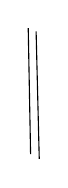
\begin{tikzpicture}\draw (0,0) -- (0.03,-1.6);\draw (0.10,-0.04) -- (0.14,-1.66);\end{tikzpicture}}}
La conjecture qui se présente tout de suite, c'est que ces deux revêtements proétales sont isomorphes -- l'isomorphisme entre les deux \unsure{est} alors unique.


\deleted{\unsure{Et}} C'est le moment de déterminer les classes d'isomorphie des \unsure{classes} de scindages de \inserted{l'ext. $\widetilde{\mathcal M}\unsure{\simeq}\mathcal M_{0,3}/[\widehat\Pi_{0,3},\widehat\Pi_{0,3}]$ de} $\Gamma=\Gamma_{\mathbb Q}\times\mathfrak S_3$ par $M^{\wedge}$, on a par la suite exacte associée à la suite spectrale de Hochschild

$(294)$\quad
\diagram{\begin{tikzcd}[ampersand replacement=\&,column sep=small]
0\arrow[r,dash]\&H^1(\Gamma_{\mathbb Q},H^0(\deleted{\unsure{\widetilde\Gamma}}\mathfrak S_3,\widehat M))\arrow[r,dash]\&H^1(\unsure{\Gamma},\widehat M)\arrow[r,dash]\&H^0(\Gamma_{\mathbb Q},H^1(\mathfrak S_3,\widehat M))\arrow[d]\\
\&\&\&H^2(\Gamma_{\mathbb Q},H^0(\mathfrak S_3,M))
\end{tikzcd}}

Or on a vu que
\[
(295)\qquad H^0(\mathfrak S_3,\widehat M)=0
\qquad(\text{\unsure{et} }\overline{\mathrm m}\ H^0(\unsure{L_\rho|L_j},\unsure{\widehat M|\overline M})=0)
\]
\margin{donc $H^1(\Gamma,\widehat M)\simeq H^0(\Gamma_{\mathbb Q},H^1(\mathfrak S_3,\widehat M))$}
\deleted{\unsure{Et}} Calculons d'autre part
\[
H^1(\mathfrak S_3,\widehat M)=H^1(\mathfrak S_3,M)\otimes_{\mathbb Z}\widehat{\mathbb Z},
\]

\margin{135}

% Archive printed footer (not manuscript):
% 135
% https://grothendieck.umontpellier.fr
% Université de Montpellier, UMR CNRS 5149, Case courrier 051, Place Eugène Bataillon
% 34095 Montpellier cedex 5 - France

\scanpage{137}
\mspage{716}

ce qui nous \unsure{ramène} à calculer
\[
H^1(\mathfrak S_3,M)\quad ?
\]
Mais l'étude faite de l'extension $\mathfrak S^+/\mu_{\mathfrak S}$ de $\mathfrak S_3$ par $M$ -- qui nous a montré que cette extension était scindée, et que deux scindages étaient conjugués par un unique élément de $M$, nous donne en fait
\[
(296)\qquad
\left\{\begin{array}{ll}
H^0(\mathfrak S_3,M)=H^1(\mathfrak S_3,M)=0&\text{d'où}\\
H^0(\mathfrak S_3,\unsure{\widehat M|\overline M})=H^1(\mathfrak S_3,\unsure{\widehat M|\overline M})=0&
\end{array}\right.
,
\]
d'où finalement, grâce à $(295)$, la relation triomphale
\[
(297)\qquad\boxed{H^1(\Gamma_{\mathbb Q}\times\mathfrak S_3,\widehat M)=0}\qquad !
\]

On trouve donc -- à nouveau contre toute attente, je l'avoue ! -- le

\uline{Théorème}\quad Il existe un \deleted{pro}revêtement
\margin{\figure{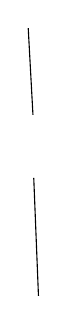
\begin{tikzpicture}\draw (0,0) -- (0.06,-1.1);\draw (0.07,-1.9) -- (0.13,-3.4);\end{tikzpicture}}}
proétale \deleted{$\unsure{X|Z}$} $U_\infty$ de $(U_{0,3\,\mathbb Q},\mathfrak S_3)$\inserted{$=M'_{1,1\,\mathbb Q}$}, ayant la propriété suivante : L'image inverse \inserted{$\overline U_\infty$} de $U_\infty$ sur $U_{0,3\,\overline{\mathbb Q}}$ (\deleted{\unsure{sans}}\inserted{\unsure{oubliant}} op. de $\mathfrak S_3$) est ``le'' revêtement abélien universel de $U_{0,3\,\overline{\mathbb Q}}$. Pour deux tels revête-

\margin{136}

% Archive printed footer (not manuscript):
% 136
% https://grothendieck.umontpellier.fr
% Université de Montpellier, UMR CNRS 5149, Case courrier 051, Place Eugène Bataillon
% 34095 Montpellier cedex 5 - France

\scanpage{138}

ments proétales de $(U_{0,3\,\mathbb Q},\mathfrak S_3)=M'_{1,1\,\mathbb Q}$, il existe un unique isomorphisme de l'un sur l'autre.

Nous avons obtenu l'existence de \uline{deux} façons : par la tour de Fermat, et par la théorie générale du \S\,$49$ \uline{III}, appliquée au cas présent -- ce qui nous donne un $U_\infty$ et un $U'_\infty$, chacun décrit à isom unique près ! Le th. d'unicité résulte du petit calcul précédent -- j'avais peur du ``gros'' \deleted{$\unsure{H^1(\Gamma_{\mathbb Q},\widehat M)\simeq H^1(\Gamma}$}
\[
H^1(\Gamma_{\mathbb Q},\widehat M)\simeq
M\otimes_{\mathbb Z}\underbrace{H^1(\Gamma_{\mathbb Q},T_{\unsure{\infty|*}}(G_m))}_{\widehat{\mathbb Q^{*}}},
\]
mais finalement c'est la nullité de $H^{i}(\mathfrak S_3,M)$ pour $i=0,1$ qui implique (sans rien connaître sur $\Gamma_{\mathbb Q}$ !) celle de $H^1(\Gamma_{\mathbb Q}\times\mathfrak S_3,\widehat M)$, qui assure l'unicité qu'il nous fallait.

\margin{137}

% Archive printed footer (not manuscript):
% 137
% https://grothendieck.umontpellier.fr
% Université de Montpellier, UMR CNRS 5149, Case courrier 051, Place Eugène Bataillon
% 34095 Montpellier cedex 5 - France

\scanpage{139}
\mspage{717}

\deleted{Car} Le théorème précédent élucide complètement, il me semble, la signification arithmético-géométrique (en termes de la tour de Fermat) de l'homomorphisme ((218) p.~695')
\[
\mathcal M=N_{1,1}^{\text{ét}}\longrightarrow G_{\rho,\sigma}\simeq\widehat{\mathbb Z}^{*}\mathbin{.}\mathfrak S_{\unsure{\bullet|0}}^{+\wedge}
\]
obtenu dans la section 11°) par voie purement algébrique --- ou du moins celui de l'homomorphisme un peu plus faible
\[
\mathcal M\longrightarrow\overbrace{G_{\rho,\sigma}/\mu_{\mathfrak S}}^{\inserted{G_{\rho,\widetilde{\sigma}}\overset{\mathrm{dfn}}{=}}}\simeq\widehat{\mathbb Z}^{*}\mathbin{.}\mathfrak S^{+\wedge}/\mu_{\mathfrak S}
\]
qui se factorise \deleted{par} en un hom
\[
\underbrace{\widetilde{\mathcal M}}_{\inserted{\text{noté }\mathcal M\text{ dans les pages précédentes}}}\overset{\mathrm{dfn}}{=}\mathcal M/(\mu_{\mathcal M}=\mu_{\mathfrak S_{\unsure{0|\bullet}}})\longrightarrow G_{\rho,\widetilde{\sigma}}
\qquad\text{extension de }\widetilde\Gamma=\widehat{\mathbb Z}^{*}\times\mathfrak S_3\text{ par }M^\wedge.
\]

Le passage de $G_{\rho,\sigma}^{\deleted{\unsure{\sim}}}$ à $G_{\rho,\widetilde{\sigma}}$, du point de vue actuel, avait comme rôle essentiel (a posteriori !) de fournir une extension par $M^\wedge$ (jouant le rôle d'une composante neutre) d'un groupe opérant \uline{fidèlement} sur $M^\wedge$, ce qui n'était pas le cas de l'ext. $G_{\rho,\sigma}$ de $\widehat{\mathbb Z}^{*}\times H^+$ par $M^\wedge$, puisque le \deleted{\unsure{centre|élément}} \inserted{centre $\mu_{H^+}=\{1,\unsure{\omega_{H^+}}\}$ \deleted{\unsure{$H^+$}} de $H^+$} opérait trivialement.
\margin{138}

% Archive printed footer (not manuscript):
% 138
% https://grothendieck.umontpellier.fr
% Université de Montpellier, UMR CNRS 5149, Case courrier 051, Place Eugène Bataillon
% 34095 Montpellier cedex 5 - France

\scanpage{140}

Ceci, joint aux relations
\[
H^0(\widehat{\mathbb Z}^{*}\times\mathfrak S_3,\widehat M)=H^1(\widehat{\mathbb Z}^{*}\times\mathfrak S_3,\widehat M)=0,
\]
permettait d'interpréter le groupe $G_{\rho,\widetilde\sigma}$ comme un groupe de transformations sur l'ens $E$ de ses propres scindages, ce qui permettait d'interpréter l'hom $\mathcal M\to G_{\rho,\widetilde\sigma}$ (ou $\widetilde{\mathcal M}\to G_{\rho,\widetilde\sigma}$) comme une \deleted{\unsure{ho}} \uline{opération} de $\mathcal M$ \deleted{\unsure{de $H$}} (ou mieux, \deleted{de $\unsure{\widetilde{\mathcal M}}$}\inserted{de $\widetilde{\mathcal M}=\pi_1(U_{0,3\mathbb Q},\mathfrak S_3)=\pi_1(M'_{1,1\mathbb Q})$} sur $E$), correspondant donc à un revêtement \inserted{proétale} de $(U_{0,3\mathbb Q},\mathfrak S_3)\simeq M'_{1,1\mathbb Q}$ --- et ce revêtement n'est autre que le prorevêtement de Fermat.

Il restait à interpréter de façon analogue l'hom $\boxed{\mathcal M=N_{1,1}\longrightarrow G_{\rho,\sigma}}$, s'insérant dans l'hom de suites exactes
\[
\tag{298}
\diagram{\begin{tikzcd}[ampersand replacement=\&,column sep=small,row sep=large]
1\arrow[r]\&\begin{gathered}\mu_{\mathcal M}\\\Vert\\(\{1,\omega\})\end{gathered}\arrow[r]\arrow[d,"\simeq"]\&\begin{gathered}\mathcal M\\\Vert\\(N_{1,1})\end{gathered}\arrow[r]\arrow[d]\&\begin{gathered}\widetilde{\mathcal M}\\\Vert\\(N'_{1,1}=\unsure{\mathcal M_{0,3}})\end{gathered}\arrow[r]\arrow[d]\&1\\
1\arrow[r]\&\begin{gathered}\mu_G\\\Vert\\\{1,\omega\}\end{gathered}\arrow[r]\&G_{\rho,\sigma}\arrow[r]\&G_{\rho,\widetilde\sigma}\arrow[r]\&1
\end{tikzcd}},
\]
\deleted{Pour} qui permet d'interpréter d'ailleurs $\mathcal M$, en tant qu'extension centrale de $\widetilde{\mathcal M}$
\margin{139}

% Archive printed footer (not manuscript):
% 139
% https://grothendieck.umontpellier.fr
% Université de Montpellier, UMR CNRS 5149, Case courrier 051, Place Eugène Bataillon
% 34095 Montpellier cedex 5 - France

\scanpage{141}
\mspage{718}

par $\mu$, comme image inverse de l'extension $G_{\rho,\sigma}$ de $G_{\rho,\widetilde\sigma}$ par $\mu$, par l'homomorphisme $\widetilde{\mathcal M}\to G_{\rho,\widetilde\sigma}$ précédent. Il y a une analogie frappante avec ce qui s'était passé, d'ailleurs, quand on était parti \unsure{de} (au \S~48, et \unsure{dans|des} certains développements qui l'ont précédé) du groupe quotient (``du type Lie'') $\unsure{\mathrm{SL}(2,\widehat{\mathbb Z})'}$ de $\unsure{\mathfrak S_{0,3}^{+\wedge}}$, pour construire un hom
\[
\deleted{\unsure{\mathcal M}}\qquad \mathcal M_{0,3}\longrightarrow\mathrm{GL}(2,\widehat{\mathbb Z})/\{\pm1\}
\]
d'où il nous a été possible de reconstituer \deleted{$\unsure{\mathcal M}$} l'ext. $\mathcal M=N_{1,1}$ de $\mathcal M_{0,3}$ par $\mu$ justement comme l'image inverse de l'extension $\mathrm{GL}(2,\widehat{\mathbb Z})$ de $\mathrm{GL}(2,\widehat{\mathbb Z})/\{\pm1\}$ par $\mu=\{\pm1\}$. Du pt de vue actuel où j'essaye d'expliciter autant que possible des aspects arithmético-géométriques en termes d'automorphismes des groupes à lacets \inserted{profinis} $\Pi_{0,3}^\wedge$ --- le fait remarquable, c'est que les deux
\margin{140}

% Archive printed footer (not manuscript):
% 140
% https://grothendieck.umontpellier.fr
% Université de Montpellier, UMR CNRS 5149, Case courrier 051, Place Eugène Bataillon
% 34095 Montpellier cedex 5 - France

\scanpage{142}

extensions de $\widetilde{\mathcal M}$ par $\mu$, sortant de calculs en apparence assez différents, soient canoniquement isomorphes.

Je présume qu'une explication générale de ce fait \unsure{n'offrira|n'offrirait} aucune difficulté, dans le contexte actuel --- du fait que dans les deux cas, le \inserted{bi-}\unsure{revêtement} de $\unsure{\mathrm{GL}|\mathrm{SL}}(2,\widehat{\mathbb Z})/\pm1$ resp de $G_{\rho,\widetilde\sigma}$ provenait du fait que j'étais parti d'un groupe quotient ($\mathrm{SL}(2,\widehat{\mathbb Z})$ ou $\mathfrak S^{+\wedge}$) \uline{non pas} de $\mathfrak S_{0,3}^{+\wedge}\simeq\mathrm{SL}(2,\mathbb Z)^\wedge/\pm1$, mais de $\mathrm{SL}(2,\mathbb Z)^\wedge\simeq N_{1,1}$ lui-$\overline{\mathrm m}$ ---

Si on cherche malgré tout une interprétation (genre ``tour de Fermat'') de l'hom $\mathcal M\to G_{\rho,\sigma}$, il faudrait interpréter $G_{\rho,\sigma}$ \inserted{(comme \unsure{l'était} $G_{\rho,\widetilde\sigma}$)} comme un groupe d'automorphismes d'une ``fibre type'' ``pas trop grosse'' --- la difficulté étant d'inventer quelque chose sur quoi \unsure{ça|il} opère de façon non triviale.
\margin{141}

% Archive printed footer (not manuscript):
% 141
% https://grothendieck.umontpellier.fr
% Université de Montpellier, UMR CNRS 5149, Case courrier 051, Place Eugène Bataillon
% 34095 Montpellier cedex 5 - France

\scanpage{143}
\mspage{719}

Interprétant $\mathcal M_{0,3}=N'_{1,1}$ comme $\pi_1(M'_{1,1})$, où $M'_{1,1}$ est le schéma modulaire/$\mathbb Q$ des courbes elliptiques à symétrie près, on voit que la tour de Fermat revient à ceci : sur tout schéma de base $S$ (disons \inserted{\uline{de car. 0}}) et \unsure{tte|tt} quasi-courbe elliptique \inserted{\deleted{$\unsure{E}$}$\widetilde X$} sur $S$, considérons le revêtement étale de degré trois $S'$ de $S$ correspondant (\inserted{des} ``pts d'ordre 2 de $\widetilde X$''), \deleted{posons} soit
\[
\tag{299}
\deleted{\unsure{M_2}}\quad M_0(\widetilde X/\unsure{S|B})\overset{\mathrm{dfn}}{=}p_*(\mathbb Z_{\unsure{S'|B'}})/\mathbb Z_S
\]
le $\mathbb Z$-module constant tordu libre de rang \deleted{trois}\inserted{deux} correspondant, et considérons
\[
\tag{300}
\deleted{\unsure{M_2}}\quad M_1(\widetilde X/S)\overset{\mathrm{dfn}}{=}M_0(\widetilde X/S)\otimes_{\mathbb Z}\underbrace{\unsure{\widehat{\mathbb Z}(1)}}_{\inserted{\begin{gathered}\Vert\,\mathrm{dfn}\\T_\infty(\mathbb G_m)\end{gathered}}},
\]
qui est un \deleted{pro}groupe proétale sur $S$, un syst de coefficients loc isom. (au sens large) à $\widehat{\mathbb Z}^{2}$. \deleted{Ceci posé,}\inserted{Bien} sûr, $M_1(\widetilde X/S)$ dépend \unsure{fonctoriellement} de $\widetilde X/S$ pour iso et images inverses (on a une section cartésienne d'une cat. fibrée ad-hoc $\ldots$). Ceci posé,
\margin{142}

% Archive printed footer (not manuscript):
% 142
% https://grothendieck.umontpellier.fr
% Université de Montpellier, UMR CNRS 5149, Case courrier 051, Place Eugène Bataillon
% 34095 Montpellier cedex 5 - France

\scanpage{144}

la donnée de la ``tour de Fermat'' équivaut à la donnée, pour $\forall\,\widetilde X/S$ comme dessus, d'un torseur
\[
\tag{301}
F_\infty(\widetilde X/S)\quad\text{torseur sur }S\text{ sous }M_1(\widetilde X/S),
\]
\margin{pour une construction géométrique cf (320) p. 724}
compatible aux iso. et \unsure{chgts} de base.

Le théorème précédent dit essentiellement qu'un tel $F_\infty(\widetilde X/S)$ existe, et est unique à iso. unique près, en exigeant de plus que l'hom naturel
\diagram{\begin{tikzcd}[ampersand replacement=\&]
\Pi_{0,3}^{\wedge}\arrow[r] \& M^{\wedge}
\end{tikzcd}}
associé à une telle donnée $F_\infty$ soit l'hom canonique $\ldots$.

Soit d'autre part $X$ une courbe elliptique relative au dessus d'une base $S$ de car. 0, et soit $S'\subset X$ le sous-schéma fermé, étale de degré 3 sur $S$, correspondant aux pts d'ordre 2. Considérons la \unsure{jacobienne généralisée} de $X$ déduite de cette multisection, soit $\mathcal J^0$ sa partie de degré 0, on a donc

\margin{143}

% Archive printed footer (not manuscript):
% 143
% https://grothendieck.umontpellier.fr
% Université de Montpellier, UMR CNRS 5149, Case courrier 051, Place Eugène Bataillon
% 34095 Montpellier cedex 5 - France

\scanpage{145}
\mspage{720}

une suite exacte
\[
\tag{302}
\diagram{\begin{tikzcd}[ampersand replacement=\&]
1\arrow[r] \& \mathcal J_0^0\arrow[r,dash]\arrow[d,phantom,"\rotatebox{90}{$\simeq$}" description] \& \mathcal J^0\arrow[r] \& X\arrow[r,dash] \& 1\\
\& \mathbb G_m\otimes_{\mathbb Z}M_0
\end{tikzcd}}
\]
où $M_0=M_0(X/S)$ est défini plus haut (299). On en déduit une suite exacte
\[
\tag{303}
\diagram{\begin{tikzcd}[ampersand replacement=\&]
1\arrow[r] \& M_1\arrow[r]\arrow[d,equal] \& T_\infty(\mathcal J^0)\arrow[r] \& T_\infty(X)\arrow[r,dash] \& 1\\
\& M_0\otimes_{\mathbb Z}T_\infty(\mathbb G_m)
\end{tikzcd}}
\]
où
\[
\tag{\uline{304}}
T_\infty(G)=\varprojlim_n {}_nG
\]
est le système local des $\Pi_1$ du schéma en groupes lisse comm. \inserted{à fibres connexes} sur $S$. Donc la donnée d'un torseur sous $M_1$ équivaut à la donnée d'un torseur sous $T_{\unsure{\infty|\alpha}}(\mathcal J^0)$, muni d'une section du torseur associé \unsure{du|de} groupe $T_\infty(X)$.
\unsure{Y-a-t-il|Y a-t-il} une description remarquable du torseur de Fermat $F_\infty(X/S)$, en termes de la géométrie de la courbe elliptique relative $X/S$ ?

\margin{144}

% Archive printed footer (not manuscript):
% 144
% https://grothendieck.umontpellier.fr
% Université de Montpellier, UMR CNRS 5149, Case courrier 051, Place Eugène Bataillon
% 34095 Montpellier cedex 5 - France

\scanpage{146}

$14^\circ)$ Relation aux jacobiennes généralisées.

Considérons la ``jacobienne généralisée'' de
\[
\inserted{U_{0,3}={}}U_{0,3\,\deleted{\unsure{\mathbb Q}}\inserted{\mathbb Z}}
=\deleted{\unsure{\mathbb A_{\mathbb Q}}}\mathbb P^1_{\deleted{\unsure{\mathbb Q}}\inserted{\mathbb Z}}
-\{0,1,\infty\}_{\deleted{\unsure{\mathbb Q}}\inserted{\mathbb Z}},
\]
c'est donc un schéma en groupes $\mathcal J^*_{U_{0,3}}=\mathcal J^*$, \unsure{augmenté|s'envoyant} vers $\mathbb Z$, s'insérant dans la suite exacte
\[
\tag{305}
\diagram{\begin{tikzcd}[ampersand replacement=\&]
1\arrow[r] \& \mathcal J^0\arrow[r]\arrow[d,phantom,"\rotatebox{90}{$\simeq$}" description] \& \mathcal J^*\arrow[r,"\deg"] \& \mathbb Z_{\inserted{S_0}\deleted{\unsure{\mathbb Q}}}\arrow[r] \& 1\\
\& \mathbb G_{mS_0}\otimes_{\mathbb Z}M_{\unsure{0|\mathbb Z}}
\end{tikzcd}},
\]
\margin{\uline{NB} $S_0\overset{\unsure{\mathrm{df}|\mathrm{dfn}}}{=}\operatorname{Spec}\mathbb Z$}
et muni d'un \deleted{homo}morphisme canonique
\[
\tag{306}
\diagram{\begin{tikzcd}[ampersand replacement=\&]
\varphi:\ U_{0,3\,\deleted{\unsure{\mathbb Q}}\inserted{\mathbb Z}}\arrow[r] \&
\underbrace{\mathcal J^1}_{\substack{\text{sous-schéma de }\mathcal J^*\\\text{image inverse de}\\\text{la section }1\text{ de }\mathbb Z_{S_0}}}
\end{tikzcd}}
\]
Les opérations de $\mathfrak S_3$ sur $U_{0,3}$ définissent par fonctorialité des opérations de $\mathfrak S_3$ sur $\mathcal J^*$, compatibles avec la structure d'extension (305), et telles que (306) commute aux opérations de $\mathfrak S_3$.
Notons que $\mathcal J^1$ est un $\mathcal J^0$-torseur et

\margin{145}

% Archive printed footer (not manuscript):
% 145
% https://grothendieck.umontpellier.fr
% Université de Montpellier, UMR CNRS 5149, Case courrier 051, Place Eugène Bataillon
% 34095 Montpellier cedex 5 - France

\scanpage{147}
\mspage{721}

même un $(\mathfrak S_3,\mathcal J^0)$-torseur (un $\mathcal J^0$-torseur sur lequel $\mathfrak S_3$ opère de façon compatible avec ses op. sur $\mathcal J^0$), donc classifié par un élément de $H^1(S_0,\mathfrak S_3;\mathcal J^0)$. Or je présume qu'on a
\[
\tag{307}
H^0(S_0,\mathfrak S_3,\mathcal J^0)=H^1(S_0,\mathfrak S_3,\mathcal J^0)=0
\]
(où
\[
\tag{308}
\left\{\begin{aligned}
S_0&=\operatorname{Spec}\mathbb Z,\quad \mathcal J^0=\mathbb G_m\times_{\mathbb Z}M\simeq\mathbb G_m^{\{0,1,\infty\}}/\mathrm{diag}\\
&\simeq\operatorname{Ker}\left(\diagram{\begin{tikzcd}[ampersand replacement=\&,column sep=small]
\mathbb G_m^{\{0,1,\infty\}}\arrow[r] \& \mathbb G_m^{\deleted{\unsure{\{0,1,\infty\}}}}\\
(x_0,x_1,x_\infty)\arrow[r,mapsto] \& \substack{\inserted{x_0\cdot x_1\cdot x_\infty}\\\deleted{\unsure{(x_1x_\infty^{-1},x_\infty x_0^{-1},x_0x_1^{-1})}}}
\end{tikzcd}}\right)
\end{aligned}\right.
\]
\margin{Attention, ce dernier isom. est obtenu \unsure{via}
\diagram{\begin{tikzcd}[ampersand replacement=\&]
(x_0,x_1,x_\infty)\arrow[r,mapsto] \& (x_1x_\infty^{-1},x_\infty x_0^{-1},x_0x_1^{-1})
\end{tikzcd}}, qui commute à $\mathfrak S_3^+$, mais \unsure{non|pas} à $\mathfrak S_3$ tout entier}

On a en effet
\[
\begin{aligned}
H^0(S_0,\mathfrak S_3;\mathcal J^0)&\simeq\left\{(x_0,x_1,x_\infty)\in\mathbb Z^{*\{0,1,\infty\}}\ \middle|\ \begin{array}{l}x_0x_1x_\infty=1\\(x_0,x_1,x_\infty)\text{ inv. par }\mathfrak S_3\end{array}\right\}\\
&=\{(x,x,x)\mid x\in\mathbb Z^{*\{0,1,\infty\}},\quad x^3=1\}\\
&=1
\end{aligned}
\]
\margin{Calcul \unsure{correct}, car il \unsure{repose sur cet} $\mathfrak S_3^+$-isom. qui n'est pas un $\mathfrak S_3$-isom., \unsure{il semble ici qu'être|il semble n'y être} besoin de $H^0(S,\mu_3)=1$, alors qu'un calcul déjà fait des \unsure{scindages} d'extensions (cf. 720) montre que $\unsure{S}$ -- sur \uline{toute} \uuline{base}
\diagram{\begin{tikzcd}[ampersand replacement=\&,column sep=small]
H^0(S,\mathfrak S_3,\mathcal J^0)\arrow[d,equal]\arrow[r,phantom,"\simeq"] \& H^1(\deleted{\unsure{S,}}\mathfrak S_3;H^0(\unsure{S|S_0},\mathcal J^0))\simeq0\quad\unsure{\Leftarrow}\\
H^0(\mathfrak S_3,H^0(S,\mathcal J^0))
\end{tikzcd}}}

(\unsure{la} seule racine \deleted{\unsure{de}} cubique de 1 dans $\mathbb Z$ (ou $\overline{\mathrm m}$ dans $\mathbb Q$) est 1. Cela établit la première relation (307). Pour la seconde, on utilise la suite spectrale

\margin{146}

% Archive printed footer (not manuscript):
% 146
% https://grothendieck.umontpellier.fr
% Université de Montpellier, UMR CNRS 5149, Case courrier 051, Place Eugène Bataillon
% 34095 Montpellier cedex 5 - France

\scanpage{148}

\diagram{\begin{tikzcd}[ampersand replacement=\&]
H^{\unsure{*|n}}(S_0,\mathfrak S_3;\mathcal J^0) \&
\overset{\inserted{E_2^{pq}=}}{H^p(\mathfrak S_3,\uline{H}^{q}(S_0,\mathcal J^0))}\arrow[l,Rightarrow]
\end{tikzcd}}
qui donne la suite exacte
\diagram{\begin{tikzcd}[ampersand replacement=\&,column sep=small]
0\arrow[r] \& H^1(\mathfrak S_3,H^0(S_0,\mathcal J^0))\arrow[r,"\unsure{\deleted{\simeq}|\simeq}"] \& H^1(S_0,\mathfrak S_3;\mathcal J^0)\arrow[r] \& H^0(\mathfrak S_3,H^1(S_0,\mathcal J^0))\arrow[d]\arrow[dl,equal]\\
\& \& \bigl(H^{\unsure{0|q}}(\mathfrak S_3,M_{\unsure{0}}\otimes_{\mathbb Z}H^1(S_0,\mathbb G_m))\bigr) \& H^2(\mathfrak S_3,H^0(S_0,\mathcal J^0))
\end{tikzcd}}

Or on a
\[
H^1(S_0,\mathcal J^0)\simeq H^1(S_0,\mathbb G_m^2)\simeq\operatorname{Pic}(\unsure{S|S_0})^2=0
\]
\margin{\uline{NB} on n'a \uline{pas} besoin de la relation $\operatorname{Pic}(S)=0$}
donc il vient
\[
H^1(S_0,\mathfrak S_3;\mathcal J^0)\simeq H^1(\mathfrak S_3,\underbrace{H^0(S_0,\mathcal J^0)}_{\substack{\deleted{(\mathbb Z^*)^{\{0,1,\infty\}}/\mathbb Z^*}\\\deleted{\simeq\mathbb Z^*\otimes_{\mathbb Z}M_0}}})
\]

Mais en fait, les calculs faits par ailleurs montrent qu'on a
\[
\tag{309}
H^0(\mathfrak S_3,M_{\unsure{0|\alpha}}\otimes_{\mathbb Z}\unsure{I|I_0})=H^1(\mathfrak S_3,M_{\unsure{0|\alpha}}\otimes_{\mathbb Z}I)=0
\]
quel que soit le $\mathbb Z$-module $I$ (p. ex. $I=\unsure{J^0|\mathcal J^0}(S)$, $S$ un schéma \unsure{quelc.|quelq.}, \inserted{ou $I=H^1(S,\mathbb G_m)=\operatorname{Pic}(S)$}), d'où finalement,
\[
\tag{\unsure{310}}
H^0(\unsure{\deleted{S_0}|S},\mathfrak S_3;\mathcal J^0)\simeq H^1(S,\mathfrak S_3,\mathcal J^0)=0
\]
pour $\forall$ schéma $S$. On trouve ainsi :

\margin{147}

% Archive printed footer (not manuscript):
% 147
% https://grothendieck.umontpellier.fr
% Université de Montpellier, UMR CNRS 5149, Case courrier 051, Place Eugène Bataillon
% 34095 Montpellier cedex 5 - France

\scanpage{149}
\mspage{722}

\uline{Proposition} Soit \deleted{$\unsure{\mathcal J}$}
$\mathcal J^0=\mathbb G_m^{\{0,1,\infty\}}/\underbrace{\mathbb G_m}_{\mathrm{diag.}}\simeq\mathbb G_m\otimes_{\mathbb Z}\unsure{M_0|M}$
Alors pour $\forall$ $(\mathfrak S_3,\mathcal J^0)$-torseur sur une base $S$ quelconque, il existe une unique trivialisation de celui-ci, i.e une unique section, invariante par les opérations de $\mathfrak S_3$.

\uline{Corollaire 1} Sur toute base $S$, il existe un unique morphisme
\[
(311)\qquad
\diagram{\begin{tikzcd}[ampersand replacement=\&]
\psi:U_{0,3\,S} \arrow[r] \& \mathcal J^0_S
\end{tikzcd}}
\]
qui soit compatible avec les opérations de $\mathfrak S_3$, et qui (via l'hom
$\mathcal J^*_S\longrightarrow\mathcal J^0_S$ \unsure{qui|que} \unsure{le|la} \unsure{factorise}, par la propriété universelle des \illegible{1} \unsure{jacobiens} généralisés) induise l'hom
$\underset{\inserted{\mathcal J^*_S}}{\mathcal J^0_S}-\mathcal J^0_S$ identique.

\margin{\uline{NB} Avec les notations de \unsure{695}, on a $U_{0,3\,S}\simeq(U_1)_S$, où $U_1\subset\mathbb G_m^3/\mathbb G_m$ est \unsure{défini} par
\[
(312)\qquad
U_1=\{(x_0,x_1,x_\infty)\in\Gamma\mathbb G_m^{\{0,1,\infty\}}\mid x_0+x_1+x_\infty=\unsure{0}\}
\quad\mathrm{mod}\ \mathrm{diag}_3\mathbb G_m.
\]}

\uline{Corollaire 3} Soit $Y$ un schéma de

\margin{148}

% Archive printed footer (not manuscript):
% 148
% https://grothendieck.umontpellier.fr
% Université de Montpellier, UMR CNRS 5149, Case courrier 051, Place Eugène Bataillon
% 34095 Montpellier cedex 5 - France

\scanpage{150}

\unsure{Brauer}-Séveri sur $S$, de dim relative $1$ (i.e. une forme de $\mathbb P^1_S$), muni d'un sous-schéma \inserted{fermé} $S'\subset Y$, étale de degré $3$ sur $S$, et soit \deleted{$\unsure{X}$} $U=Y\setminus S'$, $\mathcal J^*_{U/S}$ le jacobien généralisé, de sorte qu'on a
\[
(313)\qquad
\diagram{\begin{tikzcd}[ampersand replacement=\&,column sep=1.5em,row sep=.5em]
1 \arrow[r,no head] \& \mathcal J^0_{U/S} \arrow[r,no head] \arrow[d,phantom,"\unsure{\wr}" description] \& \mathcal J^*_{U/S} \arrow[r,no head] \& \mathbb Z_S \arrow[r,no head] \& 1 \\
\& \mathbb G_m\otimes_{\mathbb Z}\unsure{M_0}(S'/S) \& \& \&
\end{tikzcd}}
\]
où $\unsure{M_0}(S'/S)\simeq\unsure{p_*|\rho_*}(\mathbb Z_{S'})/\underbrace{\mathbb Z_S}_{\mathrm{diag}}$ est le $S$-schéma \inserted{en \deleted{groupes} \inserted{$\mathbb Z$-modules}} (loc. $\unsure{\overline{\mathrm{isom.}}}$ à $\mathbb Z^{\unsure{2}}$, déduit de $\unsure{M_{0\,S}}$ en le tordant (via action de $\mathfrak S_3$) par le \deleted{fibré principal} \inserted{$\mathfrak S_3$-torseur sur $S$} associé à $S'$.

Il existe alors un unique morphisme
\[
(\unsure{314})\qquad
\diagram{\begin{tikzcd}[ampersand replacement=\&]
\psi:U \arrow[r] \& \mathcal J^0_{U/S}
\end{tikzcd}}
\]
commutant à \deleted{$\uline{\operatorname{Aut}}$} l'action de $\uline{\operatorname{Aut}}(S'/S)\xleftarrow{\sim}\uline{\operatorname{Aut}}_S(Y,S')$, et induisant (par la propriété universelle) \deleted{\unsure{un}} l'hom. \unsure{composé}
\[
\diagram{\begin{tikzcd}[ampersand replacement=\&]
\mathcal J^0_{U/S} \arrow[r,hook] \& \mathcal J^*_{U/S} \arrow[r,"\widetilde\psi"] \& \mathcal J^0_{U/S}
\end{tikzcd}}
\]
qui soit l'identité.

\margin{149}

% Archive printed footer (not manuscript):
% 149
% https://grothendieck.umontpellier.fr
% Université de Montpellier, UMR CNRS 5149, Case courrier 051, Place Eugène Bataillon
% 34095 Montpellier cedex 5 - France

\scanpage{151}
\mspage{723}

Explicitons \unsure{le|l'} \deleted{homo}morphisme
\[
(315)\qquad
\diagram{\begin{tikzcd}[ampersand replacement=\&,column sep=2em,row sep=.9em]
U_{0,3}=\mathbb P^1\setminus\{0,1,\infty\}_{S_0}
  \arrow[r,hook,"\psi"] \arrow[d,equal]
\& \underbrace{\mathbb G_m^{\{0,1,\infty\}}/\mathbb G_m}_{\unsure{\mathcal J^0}}
\\
\begin{gathered}
\deleted{\{z\in\unsure{\Gamma}\mathbb G_m\mid z-1\ \mathrm{inv}\}}\\
\unsure{(}\mathbb G_m\setminus\{1\}\unsure{)}_{S_0}
\simeq\{z\in\Gamma\mathbb G_m\mid z-1\ \mathrm{inv}\}
\end{gathered}
\& \begin{gathered}
\deleted{\unsure{\mathcal J^1}}\inserted{U_1=\{(x_0,x_1,x_\infty)^{\deleted{\unsure{\mathbb Z}}}
\in\Gamma\mathbb G_m^3/\mathbb G_m\mid}\\
\inserted{x_0+x_1+x_\infty=0\}}
\end{gathered} \arrow[u,hook]
\end{tikzcd}}
\]
\deleted{\unsure{il}} \deleted{\unsure{c'est}} isomorphisme de $U_{0,3}$ avec $U_1$ qui \deleted{\unsure{est}} correspond : \deleted{\unsure{il faut|prolonge}}
\[
(316)\qquad
\left\{\begin{array}{l}
\diagram{\begin{tikzcd}[ampersand replacement=\&,column sep=2em,row sep=.5em]
\overline\psi:\unsure{\widehat U_{0,3}|\overline U_{0,3}} \arrow[r] \arrow[d,equal]
\& \widehat U_1\subset\mathbb P^2_{S_0} \arrow[d,equal]\\
\mathbb P^1_{S_0}
\& \{(x_0,x_1,x_\infty)\in\unsure{\widehat{\mathbb P}^2_{\unsure{S_0}}|\mathbb P^2_{S_0}}\mid x_0+x_1+x_\infty=0\}
\end{tikzcd}}\\[1em]
\overline\psi(0)=(0,1,-1)\\
\overline\psi(1)=(-1,0,1)\\
\overline\psi(\infty)=(1,-1,0)
\end{array}\right.\ ,
\]
il suffit de prendre
\[
(317)\qquad
\psi(z)=(-z,z-1,1)=(1,1/z-1,-1/z)
\inserted{=\left(\frac{-z}{z-1},1,\frac{1}{z-1}\right)}.
\]

Revenons maintenant à la donnée d'une courbe elliptique relative \inserted{$X$} sur $S$ modulo symétrie (correspondant à un morphisme
$S\longrightarrow\deleted{\unsure{\operatorname{Spec}}}\mathcal M'_{1,1}$).

\margin{150}

% Archive printed footer (not manuscript):
% 150
% https://grothendieck.umontpellier.fr
% Université de Montpellier, UMR CNRS 5149, Case courrier 051, Place Eugène Bataillon
% 34095 Montpellier cedex 5 - France

\scanpage{152}

On suppose $2$ inv. sur $S$, de sorte que la donnée de $X$ \inserted{modulo $\omega_X$} correspond, par le \unsure{tapis} de Legendre $X\mapsto(X/\deleted{\text{\unsure{modulo sym.}}}\inserted{\{1,\omega_X\}})$, à la donnée d'un $(Y,S')$ comme dessus, avec en \uline{plus} une section de $U=Y-S'$.

En fait, la donnée de $(Y,S')$ revient à la donnée de $S'$, \inserted{i.e d'un $\mathfrak S_3$-torseur} \deleted{$Y$ se récupère} $T$ sur $S$ --- et $Y$ se récupère à partir de \unsure{là|lui} comme le schéma tordu $T\wedge_{\mathfrak S_3}\mathbb P^1_S$ \deleted{$\unsure{\wedge_{\mathfrak S_3}}$ \unsure{et|ou}, $T\wedge_{\mathfrak S_3}\mathcal J^0_{(U_{0,3})_S}\simeq\unsure{\mathcal J^0}$}
avec
\[
U=Y\setminus S'\simeq(T\wedge_{\mathfrak S_3}\mathbb P^1_S)\setminus\underbrace{T\wedge_{\mathfrak S_3}\{0,1,\infty\}_S}_{S'}
\]
plongé canoniquement dans
\[
T\wedge_{\mathfrak S_3}\mathcal J^0_{(U_{0,3})_S}\simeq\mathcal J^0_{U/S}.
\]
Le plongement $U\subset\mathcal J^0_{U/S}$ peut s'interpréter aussi comme un morphisme canonique
\[
(318)\qquad
\diagram{\begin{tikzcd}[ampersand replacement=\&]
X \arrow[r] \& \mathcal J^0_{U/S}\underbrace{=\unsure{\mathcal J^0_{0\,X/S}|\mathcal J^0_{X/S}}}_{\substack{\text{\unsure{avec|en} notations}\\\text{de p. }720}}
\end{tikzcd}}
\]
qui doit être aisé à caractériser \unsure{axiomatiq}

\margin{151}

% Archive printed footer (not manuscript):
% 151
% https://grothendieck.umontpellier.fr
% Université de Montpellier, UMR CNRS 5149, Case courrier 051, Place Eugène Bataillon
% 34095 Montpellier cedex 5 - France
